%%%%%%%%%%%%%%%%%%%%%%%%%%%%%%%%%%%%%
%                                   %
% Compile with XeLaTeX and biber    %
%                                   %
% Questions or comments:            %
%                                   %
% joshua dot mcneill at uga dot edu %
%                                   %
%%%%%%%%%%%%%%%%%%%%%%%%%%%%%%%%%%%%%

\documentclass{beamer}
  % Read in standard preamble (cosmetic stuff)
  %%%%%%%%%%%%%%%%%%%%%%%%%%%%%%%%%%%%%%%%%%%%%%%%%%%%%%%%%%%%%%%%
% This is a standard preamble used in for all slide documents. %
% It basically contains cosmetic settings.                     %
%                                                              %
% Joshua McNeill                                               %
% joshua dot mcneill at uga dot edu                            %
%%%%%%%%%%%%%%%%%%%%%%%%%%%%%%%%%%%%%%%%%%%%%%%%%%%%%%%%%%%%%%%%

% Beamer settings
% \usetheme{Berkeley}
\usetheme{CambridgeUS}
% \usecolortheme{dove}
% \usecolortheme{rose}
\usecolortheme{seagull}
\usefonttheme{professionalfonts}
\usefonttheme{serif}
\setbeamertemplate{bibliography item}{}

% Packages and settings
\usepackage{fontspec}
  \setmainfont{Charis SIL}
\usepackage{hyperref}
  \hypersetup{colorlinks=true,
              allcolors=blue}
\usepackage{graphicx}
  \graphicspath{{../../figures/}}
\usepackage[normalem]{ulem}
\usepackage{enumerate}

% Document information
\author{M. McNeill}
\title[FREN2001]{Français 2001}
\institute{\url{joshua.mcneill@uga.edu}}
\date{}

%% Custom commands
% Lexical items
\newcommand{\lexi}[1]{\textit{#1}}
% Gloss
\newcommand{\gloss}[1]{`#1'}
\newcommand{\tinygloss}[1]{{\tiny`#1'}}
% Orthographic representations
\newcommand{\orth}[1]{$\langle$#1$\rangle$}
% Utterances (pragmatics)
\newcommand{\uttr}[1]{`#1'}
% Sentences (pragmatics)
\newcommand{\sent}[1]{\textit{#1}}
% Base dir for definitions
\newcommand{\defs}{../definitions}


  % Packages and settings

  % Document information
  \subtitle[Nos loisirs]{Nos loisirs}

\begin{document}
  % Read in the standard intro slides (title page and table of contents)
  \begin{frame}
    \titlepage
    \tiny{Office: % Basically a variable for office hours location
Gilbert 121\\
          Office hours: % Basically a variable for office hours
 lundi, mercredi, vendredi 10:10--11:10
}
  \end{frame}

  \begin{frame}{Annonces}
    \begin{itemize}
      \item Le devoir 2 à rendre le 23 septembre.
      \item[] \tinygloss{Homework 2 to be turned in September 23rd.}
    \end{itemize}
  \end{frame}

  \begin{frame}{Révision}
    \begin{center}
      \begin{tabular}{l | l l | l l}
  \multicolumn{5}{c}{jouer \gloss{to play}} \\
      & \multicolumn{2}{l |}{singulier} & \multicolumn{2}{l}{pluriel} \\
  \hline
  1re & je         & joue               & nous        & jouons \\
  2e  & tu         & joues              & vous        & jouez \\
  \hline
  3e  & il (masc)  &                    & ils (masc)  & \\
      & elle (fem) & joue               & elles (fem) & jouent \\
      & on         &                    &             & \\
\end{tabular}

    \end{center}
  \end{frame}

  \begin{frame}{Qu'est-ce qu'ils font?}
    \begin{columns}
      \column{0.5\textwidth}
        \begin{enumerate}
          \item Loïc est sportif.
          \item<2-> Helen est musicienne.
          \item<3-> Jean-Luc adore le cinéma.
          \item<4-> Maxime préfère les jeux de société.
          \item<5-> Trombone Shorty est fanatique de jazz.
        \end{enumerate}
      \column{0.5\textwidth}
        \begin{minipage}[t][0.6\textheight]{\linewidth}
          \only<1>{
            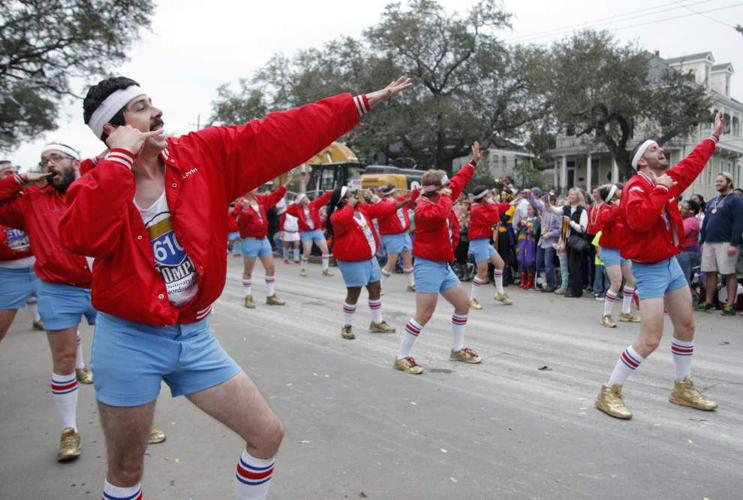
\includegraphics[scale=0.5]{stompers.jpg}
          }
          \only<2>{
            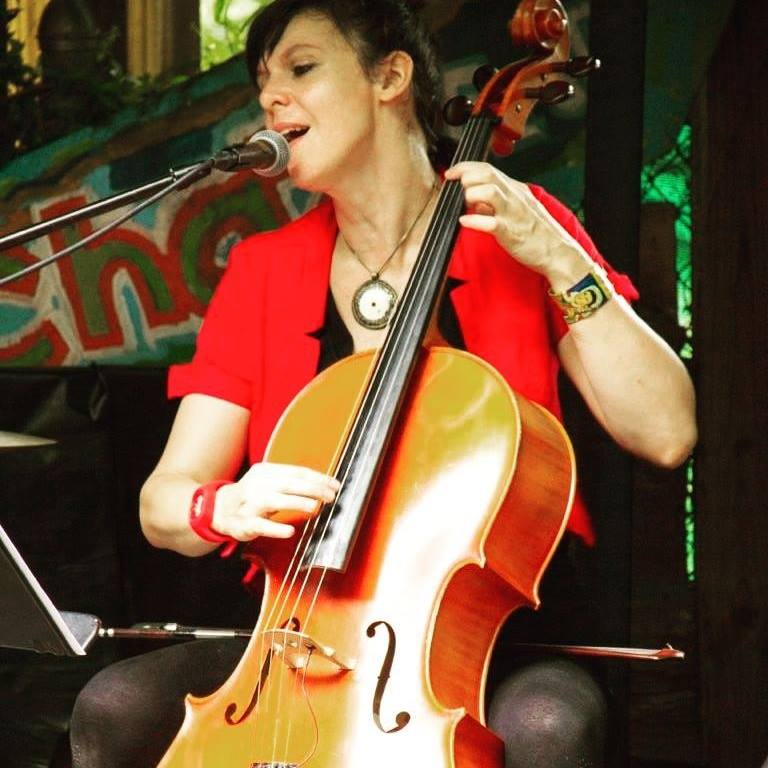
\includegraphics[scale=0.5]{helen_gillet.jpg}
          }
          \only<3>{
            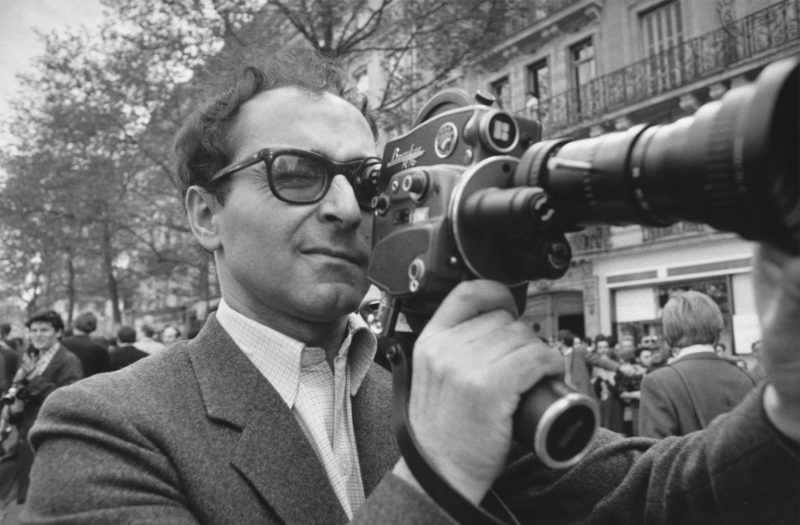
\includegraphics[scale=0.5]{godard.jpg}
          }
          \only<4>{
            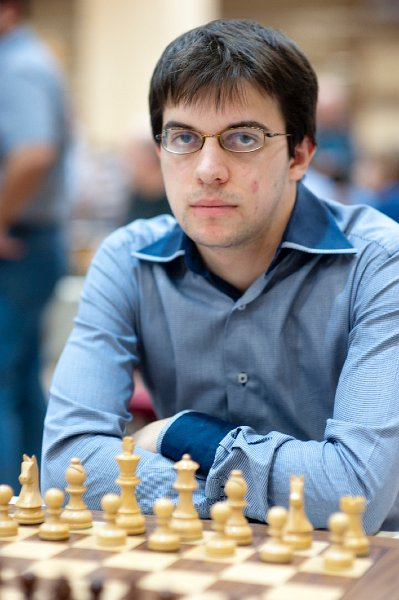
\includegraphics[scale=0.5]{maxime_vachier-lagrave.jpg}
          }
          \only<5>{
            \includegraphics[scale=0.5]{tombone_shorty.jpg}
          }
        \end{minipage}
    \end{columns}
  \end{frame}

  \begin{frame}{}
    \begin{center}
      \Large Quiz
    \end{center}
  \end{frame}

  \begin{frame}{Liaisons}
    Est-ce que vous entendez une liaison?
    \begin{columns}
      \column{0.5\textwidth}
        \begin{enumerate}
          \item nous avons \underline{\uncover<2->{oui}}
          \item des colocataires \underline{\uncover<3->{non}}
          \item chez nous \underline{\uncover<4->{non}}
          \item chez elles \underline{\uncover'5->{oui}}
          \item ils arrivent \underline{\uncover<6->{oui}}
        \end{enumerate}
      \column{0.5\textwidth}
        \begin{enumerate}
          \setcounter{enumi}{5}
          \item les yeux bleus \underline{\uncover<7->{oui}}
          \item très intelligent \underline{\uncover<8->{oui}}
          \item nos copains \underline{\uncover<9->{non}}
          \item un harmonica \underline{\uncover<10->{oui}}
          \item les cheveux noirs \underline{\uncover<11->{non}}
        \end{enumerate}
    \end{columns}
  \end{frame}

  \begin{frame}{Deux vérités et un mensonge \gloss{Two truths and a lie}}
    En groupes de 3 à 5, dites deux vérités et un mensonge par rapport à vous, à chacun son tour, et faites deviner lequel est le mensonge à vos camarades. \\
    \tinygloss{In groups of 3 to 5, take turns telling two truths and one light about yourself, and have your groupmates guess which one is the lie.} \\
    \textbf{Modèle} \\
    \begin{description}
      \item[E1:] J'ai 20 ans, je joue au rugby et j'ai des sœurs.
      \item[E2:] Tu n'as pas 20 ans?
      \item[E1:] Si, j'ai 20 ans.
      \item[E3:] Tu ne joue pas au rugby?
      \item[E1:] Oui, c'est le mensonge.
    \end{description}
  \end{frame}

  \begin{frame}{}
    \begin{center}
      \Large Questions?
    \end{center}
  \end{frame}
\end{document}
